\documentclass[tikz,border=2mm]{standalone}
\usetikzlibrary{circuits.logic.US, positioning}

\begin{document}
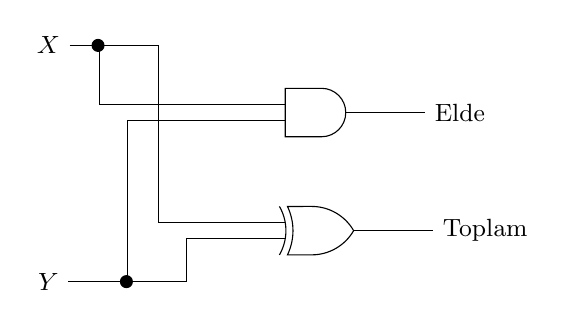
\begin{tikzpicture}[circuit logic US, every node/.style={font=\small}, 
  x=1.5cm, y=1.5cm]

  % Input nodes
  \node (i0) at (0,2) {$X$}; 
  \node (i1) at (0,0) {$Y$}; 

  % Gates
  \node [and gate, anchor=input 1] (a1) at (2,1.5) {}; % AND gate
  \node [xor gate, anchor=input 1] (x1) at (2,0.5) {}; % XOR gate

  % Output nodes
  \node [right=of a1.output] (o1) {Elde}; % Carry output
  \node [right=of x1.output] (o2) {Toplam}; % Sum output

  % Draw lines with 90-degree angles
  \draw (i0.east) -- ++(right:0.25) |- (a1.input 1); % A to AND
  \draw (i1.east) -- ++(right:0.5) |- (a1.input 2); % B to AND
  \draw (i0.east) -- ++(right:0.75) |- (x1.input 1); % A to XOR
  \draw (i1.east) -- ++(right:1) |- (x1.input 2); % B to XOR
  
  \draw (a1.output) -- ++(right:0.5) -- (o1.west); % AND to Carry output
  \draw (x1.output) -- ++(right:0.5) -- (o2.west); % XOR to Sum output

  \draw [black,fill=black] (0.42,2) circle (.5ex);
  \draw [black,fill=black] (0.66,0) circle (.5ex);
\end{tikzpicture}
\end{document}
